\setcounter{chapter}{0}

\boilerplatechapterone{%

Spacecraft trajectories and dynamics around massive gravitational bodies (planets)
are often propagated in planet centered inertial frames, which are located
at the center of the planet and have a constant orientation.
These trajectories and dynamics, however, can also depend on
models (such as atmospheric and gravitational models) requiring information
based in a planet centered planet fixed frame. Converting from a
planet centered inertial frame to a planet centered planet fixed frame requires
a matrix rotation, referred to in this document as a planet rotation model.

Often these planet rotation models
are represented as up to four individual matrix operations. These operations
account for the concepts of precession, nutation, polar offset and rotation,
referred to in this document as the Rotation, Nutation and Precession Model,
or the RNP Model.

This document presents a generic implementation for planet orientation models,
which creates a standard interface to the orientation portion of the JEOD
Ephemerides Model. It also presents a generic implementation of RNP, built
on the planet orientation interface. This allows for the reuse of basic
code common to planet orientation models formulated in the RNP
paradigm.

The generic RNP framework has also been used to create both a specific model
for the standard Earth epoch of J2000, and a specific model to represent
Mars RNP for the same J2000 epoch.
The capability to compute spacecraft trajectories in a coordinate system
defined by the mean equator and the equinox of the standard epoch of J2000
is a fixed requirement. The J2000 system is based on the position of far
away stars in the J2000 system. The implementation is a collection
of functions that compute the rotation, nutation, precession and polar motion
from the J2000 (FK5) frame to obtain the Earth Centered Earth Fixed (ECEF)
coordinate system. This document will also describe this
specific implementation of the \ModelDesc\ which, of course, takes advantage of
the \JEODid\ reuseable software framework, developed for
implementations of the RNP Earth and Mars attitude models.
} {%
   \ModelHistory
}


%----------------------------------
\chapter{Product Requirements}\hyperdef{part}{reqt}{}\label{ch:reqt}
%----------------------------------
This chapter will describe the requirements for the \ModelDesc.

\requirement{Top-level}
\label{reqt:toplevel}
\begin{description}
\item[Requirement:]\ \newline
  This model shall meet the JEOD project requirements specified in
  the \JEODid\
  \hyperref{file:\JEODHOME/docs/JEOD.pdf}{part1}{reqt}{ top-level
  document}.
\item[Rationale:]\ \newline
  This model shall, at a minimum,  meet all external and internal requirements
  applied to the \JEODid\ release.
\item[Verification:]\ \newline
     Inspection
\end{description}

\section{Data Requirements}\label{sec:data_reqts}

This section identifies requirements for the data
represented by the \ModelDesc. These as-built requirements are
based on the \ModelDesc\ data definition header files.

\requirement{Earth RNP Data Requirement}\label{reqt:earth_RNP_data}
\begin{description}
  \item[Requirement:]
The \ModelDesc\ shall encapsulate data to facilitate
the transformation from base J2000 inertial Earth coordinates
into WGS-84 Earth Centered Earth Fixed coordinates. The RNP Model
shall also encapsulate data to enable the inclusion of a polar offset
if higher fidelity is required. Finally, each component of the RNP Model
(Rotation, Nutation, Precession, Polar Motion) shall be available
as a separate matrix.
  \item[Rationale:]
The data generated by the \ModelDesc\ are the Earth Centered Earth Fixed (ECEF)
coordinates fitted to the coordinate system listed in the requirement above.
The state vector of a vehicle is generally given in an inertial coordinate
system (J2000), and geopotential gravitational accelerations are
computed in the ECEF system, thus the \ModelDesc\ must transform between
the two sets of coordinates.
  \item[Verification:]\ \newline
Unit tests are described in the \ModelDesc\ validation chapter. The verifiable
parameters should agree to as many decimal places as those presented in the
validation data from the benchmark documents Satellite Orbits,
Montenbruck and Gill \cite{MG} and Fundamentals of Astrodynamics and
Applications, Second Edition, Vallado~\cite{VMcC}.  Metric measuring of
the modeling contributions to radial, cross track, and in-track errors
is given in the \JEODid\ Top Level Document \cite{dynenv:JEOD}.
\end{description}

\requirement{Mars RNP Data Requirement}\label{reqt:mars_RNP_data}
\begin{description}
  \item[Requirement:]
The \ModelDesc\ shall encapsulate data to facilitate
the transformation from base J2000 inertial Mars coordinates
into Pathfinder Mars Centered Mars Fixed coordinates. Each component of the
RNP Model (Rotation, Nutation, Precession, Polar Motion) shall be available
as a separate matrix.
  \item[Rationale:]
The data generated by the \ModelDesc\ are the Mars Centered Mars Fixed (MCMF)
coordinates fitted to the coordinate system listed in the requirement above.
The state vector of a vehicle is generally given in an inertial coordinate
system (J2000), and geopotential gravitational accelerations are
computed in the MCMF system, thus the \ModelDesc\ must transform between
the two sets of coordinates.
  \item[Verification:]\ \newline
Verification of this requirement is by inspection.
\end{description}

\section{Functional Requirements}

This section identifies requirements on the functional capabilities provided
by the \ModelDesc.  These as-built requirements are based on the \ModelDesc\ source files.
See math model section in the specification chapter.

\requirement{Earth RNP Functional Requirement}\label{reqt:earth_RNP_func}
\begin{description}
  \item[Requirement:]\ \newline
The RNP Model shall provide the functionality to convert from the Earth J2000
inertial reference frame to WGS-84 Earth Centered Earth Fixed coordinates.
  \item[Rationale:]\ \newline
The purpose of the J2000 implementation of the
\ModelDesc\ is to provide the Earth fixed
coordinates used in many orbital dynamics routines.
  \item[Verification:]\ \newline
Unit tests are described in the \ModelDesc\ Verification and
Validation chapter. The verifiable
parameters should agree to as many decimal places as the
validation data presented in the benchmark documents Satellite Orbits,
Montenbruck and Gill~\cite{MG} and Fundamentals of Astrodynamics and
Applications, Second Edition, Vallado~\cite{VMcC}.
Metric measuring of the modeling contributions to radial, cross track,
and in-track errors is given in the \JEODid\ Top Level Document
\cite{dynenv:JEOD}.
\end{description}

\requirement{Mars RNP Functional Requirement}\label{reqt:mars_RNP_func}
\begin{description}
  \item[Requirement:]\ \newline
The RNP Model shall provide the functionality to convert from the Mars J2000
inertial reference frame into Pathfinder Mars Centered Mars Fixed coordinates.
  \item[Rationale:]\ \newline
The purpose of the RNPMars implementation of the
\ModelDesc\ is to provide the Mars fixed
coordinates used in gravitational and other orbital dynamics routines.
  \item[Verification:]\ \newline
Verification of this requirement is by inspection, since virtually all
underlying calculations of this model extension are verified as part of the
Earth J2000 implementation verification.
\cite{dynenv:JEOD}.
\end{description}

\requirement{Planet Orientation Extensibility}\label{reqt:Planet_Orientation_extension}
\begin{description}
\item[Requirement:]\ \newline
The JEOD \ModelDesc\ shall provide a standard interface to
the JEOD Ephemerides model, which can be used for implementing planet orientation
schemes based on arbitrary formulations.
\item[Verification:]\ \newline
The verification for this requirement will be done by inspection.
\end{description}

\requirement{RNP Extensibility}\label{reqt:RNP_extension}
\begin{description}
\item[Requirement:]\ \newline
The JEOD \ModelDesc\ shall provide an extensible framework appropriate for implementing orientation
schemes based on the rotation, nutation, precession and polar motion framework.
\item[Rationale:]\ \newline
The J2000 representation of RNP is not the only one in existence, and new and better implementations
are being developed that JEOD will likely incorporate in the future.
\item[Verification:]\ \newline
The verification for this requirement will be done by inspection.

\end{description}
%%% Format for the model Requirements is open.  It should include requirements for this model
%%% only and use requirment tags like the one below.
%\requirement{...}
%\label{reqt:...}
%\begin{description}
%  \item[...]\ \newline
%    The documentation for the model shall include
%
%    \subrequirement{}
%    \label{reqt:...}
%      Software requirements specification.
%
%    ...
%
%  \item[title]\ \newline
%    text
%
%  ...
%
%\end{description}

%----------------------------------
\chapter{Product Specification}\hyperdef{part}{spec}{}\label{ch:spec}
%----------------------------------

\section{Conceptual Design}

This section will present the conceptual design for the general
\ModelDesc\ framework, the J2000 (FK5) specific implementation, and the Mars
specific implementation.

\subsection{General Framework}

The general framework for the \ModelDesc\ is made up of four generic classes:

\begin{itemize}
\item{The generic planet orientation class}, which provides an interface to
the DynManager class intended for the implementation of a planet fixed
frame with respect to the planet's inertial frame,
\item{The generic RNP class}, which takes generic nutation, rotation,
precession and polar motion matrices and combines them in the correct manner,
\item{The generic planet rotation class}, the base class for any version
of a nutation, rotation, precession or polar motion matrix,
\item{A generic initialization class for planet rotations}, a base class for
any class used to initialize a planet rotation class.
\end{itemize}

The generic planet orientation class interfaces with the DynManager class
by implementing a planet orientation specific version of the EphemerisInterface
class. This class provides an interface for any object intending to interact with a DynManager
for the purpose of controlling a planet's orientation. It provides most of the virtual
function implementations necessary to instantiating a concrete version of the EphemerisInterface.
It also provides common tools necessary for interacting with the DynManager. Further
information about the DynManager \cite{dynenv:DYNMANAGER} and the EphemerisInterface
\cite{dynenv:EPHEMERIDES} can be found in their respective documents.

The generic RNP class contain implementation generic to all planet RNP formulations;
the containment of nutation, rotation, precession and polar motion objects (which can
be turned off for formulations without this component),
the algorithms for combining them, and member and utility functions
common to the individual planet rotations that make up the complete RNP rotation.

The remaining classes, the planet rotation class and its initializer, provide
tools common to rotation matrices used to implement the major components
of an RNP model. Additionally, these rotation classes can more broadly be used
to implement many other components of a planet orientation model needing
rotation matrices.

This generic framework is designed to work in concert with the \JEODid\
Time Representations Model, and the \JEODid\ Dynamics Manager. More information on these
models can be found in the Time Representations Model documentation \cite{dynenv:TIME} and the
Dynamics Manager documentation \cite{dynenv:DYNMANAGER}.

\subsection{J2000 / FK5 Specific Implementation}

The specific implementation of RNP that transforms from the J2000 ECI frame
to the ECEF frame is an implementation of the IAU-76/FK5. Further information
about this specification can be found in \cite{Bond1} and \cite{ValladoThird}.

\subsection{Mars Pathfinder Specific Implementation}

The specific implementation of RNP that transforms from the J2000 MCI frame
to the MCMF frame is an implementation named for the Mars Pathfinder mission
for which it was first used. The Pathfinder Mars RNP model is described in
\cite{Konopliv06} and \cite{Konopliv10}.

\section{Mathematical Formulations}

The ultimate product of the \ModelDesc\ is the transformation from a
planet centered inertial frame to a planet centered planet fixed frame. For
Earth, this transformation is from the Earth Centered Inertial (ECI) frame
defined by the standard epoch J2000, to the Earth Centered Earth Fixed (ECEF)
frame, as defined by the World Geodetic System 1984 \cite{WGS84}. The
transformation from planet inertial to planet centered planet fixed is often
broken into four parts: rotation, nutation, precession and polar motion. This
section will give a mathematical basis for the meaning of these separate
transformations, using the Earth RNP transformations to illustrate.

In this discussion the reader may find the following definitions
helpful:

\textbf{Definitions:}

\textbf{Luni-Solar Precession} - 50'' per year, period of $\sim $26,000
years (due to the torques of the Moon and the sun on
the Earth's equatorial bulge).

\textbf{Planetary Precession} - precession of 12''/century and
decrease of the obliquity of the ecliptic of 47''/century
(due the planetary perturbations on the Earth's orbit,
causing changes in the ecliptic).

$\zeta _A ,Z_A ,\theta _A $ are Euler angles representing the
precession of the mean celestial ephemeris pole with respect to
the space-fixed coordinate system defined by the J2000 epoch.
See figure \ref{fig:prec}. \\ \\
\textbf{Nutation} - amplitude 9'', occurs at orbital periods of
the sun and the moon (13.7 days, 27.6 days, 6 months,
1 year, 18.6 years, etc.) 18.6 year motion is largest - 20
arc sec amplitude (0.5 km).
$\varepsilon$ = The mean obliquity of the ecliptic.
$\Delta \psi$ = Nutation in longitude
$\Delta \varepsilon$ = Nutation in the obliquity.
See figure \ref{fig:nut}

\textbf{Polar Motion Linear} - drift of the rotation pole of 3-4 milli arc
seconds/year in a direction between Greenland and Hudson Bay (due to
post glacial rebound).  Long period wobble (30 years) of amplitude
30 milli arc seconds.

\textbf{Annual Wobble} - (amplitude of 0.1 arc seconds - 3
meters on the Earth's surface), 75{\%} caused by annual
variation in the inertia tensor of the atmosphere, rest
by mass variations in snow, ice, ground water, etc.
Chandler Wobble (430 day period), 6 meters amplitude.
Normal mode of the Earth. Caused by atmospheric and oceanic effects.

\textbf{Equator} - the great circle on the surface of a body formed by the
intersection of the surface with the plane passing through the center of the
body perpendicular to the axis of rotation.

\textbf{Celestial Equator} - the projection onto the celestial sphere
of the Earth's equator.

\textbf{Ecliptic} - the plane of the Earth's orbit about the sun,
affected by planetary precession.

\textbf{True Equator and Equinox of Date} - the celestial coordinate system
determined by the instantaneous positions of the celestial equator and
ecliptic (motion due to precession and nutation).

\textbf{Mean Equator and Equinox of Date} - the celestial reference system
determined by ignoring small variations of short period (nutation) in the
motions of the celestial equator (motion due to only precession).

\textbf{Mean Equator and Equinox of J2000.0} - the celestial reference system
at 12 hours, January 1, 2000.\newline

The version of RNP used
in \JEODid, found in \cite{ValladoThird} for Earth and \cite{Konopliv06} for
Mars, transforms a vector from the planet centered planet fixed frame to the
J2000 planet centered inertial frame in the following manner:

\begin{equation}\label{base_rnp_transform}
\vec{r}_{ECI} = {\bf P} * {\bf N} * {\bf R} * {\bf PM} * \vec{r}_{ECEF}
\end{equation}

where

\begin{itemize}
\item $\vec{r}_{ECI}$ is a position vector in the ECI frame,
\item $\vec{r}_{ECEF}$ is the same position vector rotated into the ECEF frame,
\item ${\bf P}$ is the matrix associated with precession,
\item ${\bf N}$ is the matrix associated with nutation,
\item ${\bf R}$ is the matrix associated with rotation, and
\item ${\bf PM}$ is the matrix associated with polar motion.
\end{itemize}

These are transformation matrices, making the writing of an equivalent transform
from J2000 planet centered inertial frame to the planet centered planet fixed
frame simple, and shown below:

\begin{equation}\label{backwards_rnp_transform}
\vec{r}_{ECEF} = {\bf PM^T} * {\bf R^T} * {\bf N^T} * {\bf P^T} * \vec{r}_{ECI}
\end{equation}

This collection of matrices is the full transform from planet centered inertial
to planet centered planet fixed coordinates, and is
referred to in this document as the ${\bf RNP}$ matrix, defined below:

\begin{equation}\label{rnp_definition}
{\bf RNP} = {\bf PM^T} * {\bf R^T} * {\bf N^T} * {\bf P^T}
\end{equation}


The following sections will describe the mathematical formulation for each
of these separate matrices. Note that the Mars Pathfinder RNP matrices are
constructed similarly, but using different parameters and slightly different
equations.

\subsection{Precession}

The J2000 Precession matrix transforms a vector from the Mean Equator
and Equinox of Date (MOD) to the mean of
equator and equinox of epoch J2000. This transformation is represented by
three consecutive single axis rotations, as shown below in
\ref{fig:prec}.

\begin{figure}[H]
\begin{center}
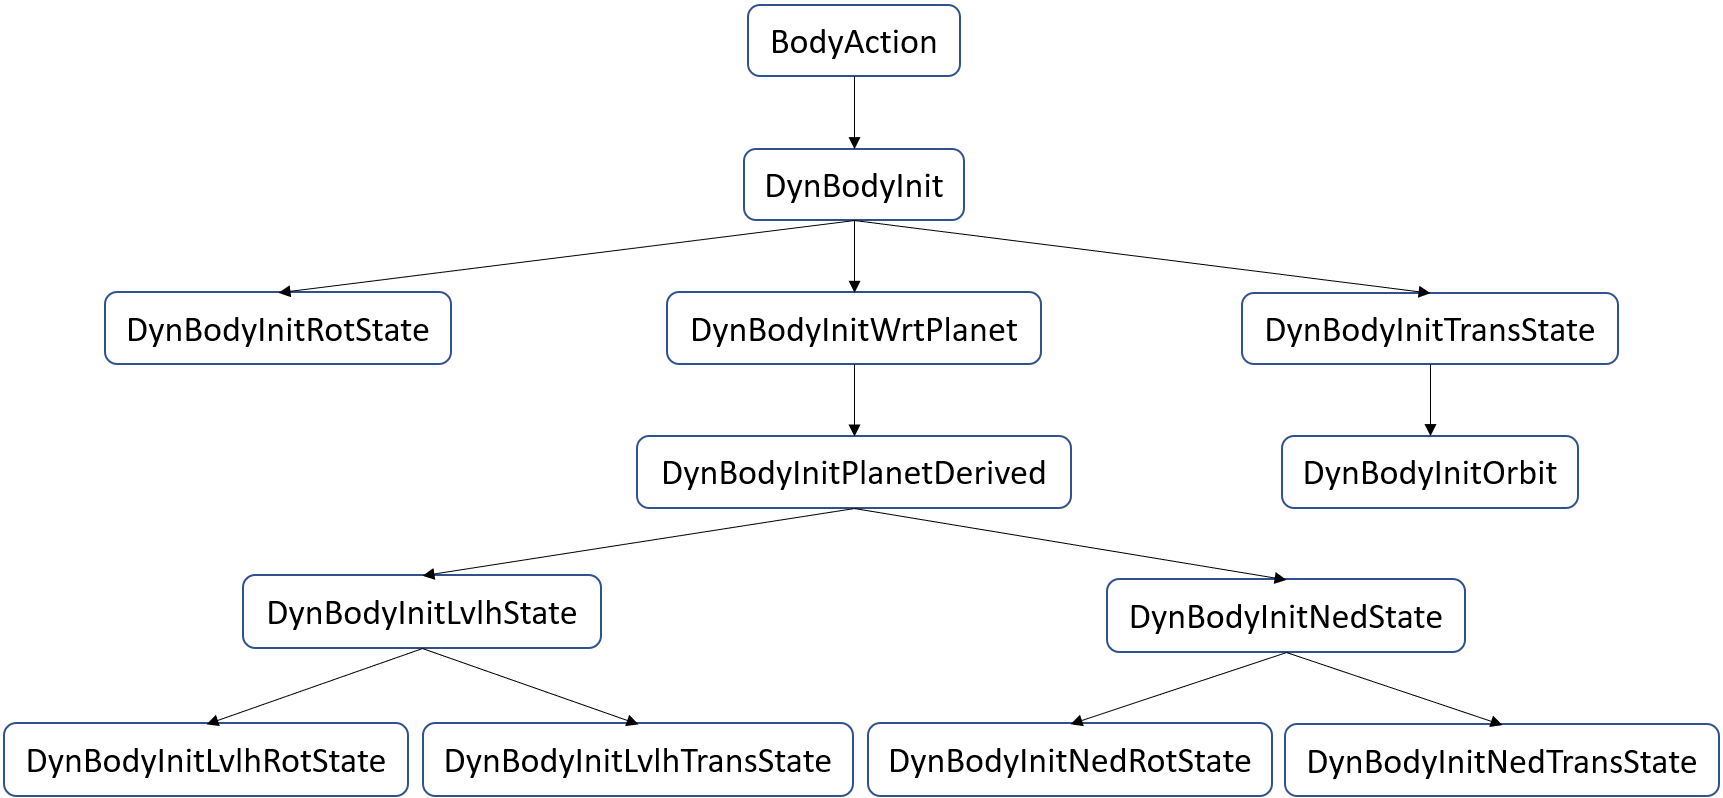
\includegraphics[height=150mm ,width = 150mm]{fig/fig1.jpg}
\caption{Rotation from the mean of equator and
equinox of epoch J2000 to Mean Equator and Equinox of Date (MOD) \cite{Bond1}}
\label{fig:prec}
\end{center}
\end{figure}

These three angles are represented as $\zeta$, $\Theta$, and z. These
values are calculated using Terrestrial Dynamic Time, which is further explained
in the \JEODid\ Time Representations Model documentation \cite{dynenv:TIME}. Terrestrial
time, indicated here as TT, is then transformed into centuries since the
J2000 epoch through the following relationship:

\begin{equation}\label{tt_centuries_since}
T_{TT} = \frac{TT - 2451545.0}{36525}
\end{equation}

where

\begin{itemize}
\item TT is the Julian Date in Terrestrial Dynamic Time, and
\item $T_{TT}$ is the number of Julian Centuries, in Terrestrial
Dynamic Time, since the J2000 Epoch.
\end{itemize}

The three angles are then calculated, according to Vallado \cite{ValladoThird},
as:

%\begin{equation}\label{tt_centuries_since}
\begin{align}\label{precession_angles}
\zeta &= 2306.2181" * T_{TT} + 0.30188 * T^2_{TT} + 0.017998 * T^3_{TT} \\
 \Theta &= 2004.3109" * T_{TT} + 0.42665 * T^2_{TT} + 0.041833 * T^3_{TT} \\
 z &= 2306.2181" * T_{TT} + 1.09468 * T^2_{TT} + 0.018203 * T^3_{TT}
\end{align}
%\end{equation}

% \begin{equation}\label{true_polar_motion_rot}
% {\bf PM} =
%  \left( \begin{array} {ccc}
% \cos x_p            & 0         & -\sin x_p \\
% \sin x_p * \sin y_p & \cos y_p  & \cos x_p * \sin y_p  \\
% \sin x_p * \cos y_p & -\sin y_p & \cos x_p * \cos y_p \end{array} \right)
% \end{equation}

The precession matrix is then formed in the following manner, per
Vallado \cite{ValladoThird}:

\begin{equation}\label{precession_matrix}
{\bf P} =
\left( \begin{array} {ccc}

\cos \Theta *  \cos z *  \cos \zeta - \sin z * \sin  \zeta
& \sin z * \cos \Theta * \cos \zeta + \sin \zeta * \cos z
& \sin \Theta * \cos \zeta \\

-\sin \zeta * \cos \Theta * \cos z - \sin z * \cos \zeta
& -\sin z * \sin \zeta * \cos \Theta + \cos z * \cos \zeta
& -\sin \Theta * \sin \zeta \\

-\sin \Theta * \cos z
& -\sin \Theta * \sin z
& \cos \Theta

\end{array} \right)
\end{equation}



\subsection{Nutation}

The J2000 Nutation matrix transforms a vector from the True Equator and Equinox
of date (TOD) to the Mean Equator
and Equinox of Date (MOD). This transformation is represented by
three consecutive single axis rotations, as shown below in
\ref{fig:nut}.


The J2000 Nutation matrix, similar to the Precession matrix, is based on three
angles, defined in \cite{Bond1} as:

\begin{itemize}
\item $\epsilon$: The mean obliquity of the ecliptic,
\item $\Delta\Psi$: The nutation in longitude, and
\item $\Delta\epsilon$: The nutation in obliquity
\end{itemize}

\begin{figure}[H]
\begin{center}
\includegraphics[height=150mm ,width = 150mm]{fig/fig2.jpg}
\caption{Rotation from Mean Equator and Equinox of Date (MOD) to
True Equator and Equinox of date (TOD) \cite{Bond1}}
\label{fig:nut}
\end{center}
\end{figure}

Additionally, \cite{Bond1} defines the relationship:

\begin{equation}\label{true_obliquity}
\epsilon^{\prime} = \epsilon + \Delta\epsilon
\end{equation}

Where $\epsilon^{\prime}$ is the true obliquity of the ecliptic.

Similar to precession, the nutation matrix is dependent on the centuries
since the J2000 epoch calculated using Terrestrial Dynamic Time. This
calculation is explained in the previous section, and shown in Equation
\ref{tt_centuries_since}.

$\epsilon$ is then calculated as a polynominal in $T_{TT}$:

\begin{equation} \label{mean_obliquity_formula}
\epsilon = 84381.448"  - 46.8150 * T_{TT} - 0.00059 * T^2_{TT} + 0.001813 * T^3_{TT}
\end{equation}

The nutation in longitude and nutation in obliquity are then calculated using
trigonometric series. These formulations are long and complex, and the full
details will not be presented here. These formulations in full can be found
in \cite{Bond1}.

The nutation matrix is then computed in the following manner, using the
calculated angles, as follows \cite{Bond1}:

\begin{equation}\label{nutation_matrix}
{\bf N} =
\left( \begin{array} {ccc}

\cos \Delta\Psi
& \cos \epsilon^{\prime} * \sin \Delta\Psi
& \sin \epsilon^{\prime} * \sin \Delta\Psi \\

-\sin \Delta\Psi * \cos \epsilon
& \cos \epsilon^{\prime} * \cos \Delta\Psi * \cos \epsilon + \sin \epsilon^{\prime} + \sin \epsilon
& \sin \epsilon^{\prime} * \cos \Delta\Psi * \cos \epsilon - \cos \epsilon^{\prime}* \sin \epsilon \\

-\sin \Delta\Psi * \sin \epsilon
& \cos \epsilon^{\prime} * \cos \Delta\Psi * \sin \epsilon - \sin \epsilon^{\prime} * \cos \epsilon
& \sin \epsilon^{\prime} * \cos \Delta\Psi * \sin \epsilon + \cos \epsilon^{\prime} * \cos \epsilon

\end{array} \right)
\end{equation}

Note that, while the notation of \cite{Bond1} is used, the matrix represented in
\eqref{nutation_matrix} is the transpose of what is shown in \cite{Bond1}, which
for the ortho-normal transformation matrix is of course the inverse of the
original matrix. This is a result of \cite{ValladoThird}
using a different formulation for the relationship between the J2000 ECI frame
and the ECEF frame, as shown in \ref{base_rnp_transform}, where the rotation,
nutation, rotation and polar motion matrices have been transposed and moved
to the opposite side. The end formulations and results,
however, are completely equivalent.


A graphical representation of the effects of nutation and precession can be
seen below in \ref{fig:nut_and_prec}.

\begin{figure} [H]
\begin{center}
\label{fig:nut_and_prec}
\includegraphics {fig/rnpfig2.jpg}
\caption{The effects of nutation and precession on the Earth
rotation axis.\cite{ValladoThird}}
\end{center}
\end{figure}
\subsection{Rotation}

The rotation matrix contained in the RNP formulation represents the sidereal
rotation of the Earth. This is the major, axial rotation of the Earth, and is
the largest contributor to the Earth orientation.

The rotation matrix is calculated from Greenwich Mean Sidereal Time, which
is further explained in the \JEODid\ Time Representations Model documentation \cite{dynenv:TIME}.
This time is then converted to an angle, as described in \cite{ValladoThird},
using the following relationship:

\begin{equation} \label{GMST_time_to_angle}
\theta_{GMST} = \frac{T_{GMST}}{240}
\end{equation}

This angle is known as the Greenwich Apparent Sidereal Time, and is
calculated using the following relationship \cite{ValladoThird}:

\begin{equation} \label{GAST_formula}
\theta_{GAST} = \theta_{GMST} + \Delta\Psi * \cos \epsilon^{\prime}
\end{equation}

where $\cos \epsilon^{\prime}$ is known as the equation of the equinoxes.

This angle is then converted to a rotation matrix through the following
relationship:

\begin{equation}\label{rotation_matrix}
{\bf R} =
\left( \begin{array} {ccc}

\cos \theta_{GAST}
& -\sin \theta_{GAST}
& 0.0 \\

\sin \theta_{GAST}
& \cos \theta_{GAST}
& 0.0 \\

0.0
& 0.0
& 1.0

\end{array} \right)
\end{equation}

\subsection{Polar Motion}

The J2000 polar motion is based on a table of values for angular displacements of
the axis of rotation of the planet. These displacements represent angular
displacements of the pole in the $x_p$ direction (positive along the direction
of the Prime Meridian), and the $y_p$
direction (positive along the $90^{\circ}$W
meridian. Thus, the rotation matrix based on these angular displacements,
as represented in \cite{ValladoThird} is:


\begin{equation}\label{true_polar_motion_rot}
{\bf PM} =
 \left( \begin{array} {ccc}
\cos x_p            & 0         & -\sin x_p \\
\sin x_p * \sin y_p & \cos y_p  & \cos x_p * \sin y_p  \\
\sin x_p * \cos y_p & -\sin y_p & \cos x_p * \cos y_p \end{array} \right)
\end{equation}

Because $x_p$ and $y_p$ are extremelly small, this matrix is often simplified to:

\begin{equation}\label{simple_polar_motion_rot}
{\bf PM} =
 \left( \begin{array} {ccc}
1            & 0         & -x_p \\
0 & 1  & y_p  \\
x_p & -y_p & 1 \end{array} \right)
\end{equation}

\section{Detailed Design}

\subsection{Planet Orientation Class}

The PlanetOrientation class implements an inheriting class of the
EphemerisInterface model. This implementation intends to provide
an EphemerisInterface for controlling a planet's orientation.
The exact details of the EphemerisInterface class and how it interacts with
the EphemerisManager portion of the DynManager can be found here \cite{dynenv:EPHEMERIDES}.

The PlanetOrientation provides implementations of the following
EphemerisInterface functions:

\begin{itemize}
\item{ephem\_initialize,}
\item{ephem\_activate, and}
\item{ephem\_build\_tree.}
\end{itemize}

"name", "timestamp", "ephem\_update" and "get\_name"
are all left to the inheriting class.

The PlanetOrientation class also provides tools for interacting with
the DynManager \cite{dynenv:DYNMANAGER}.
This includes providing tools for turning a PlanetOrientation model
on and off and instantiating an EphemerisOrientation
object \cite{dynenv:EPHEMERIDES}, intended to control the planet orientation
in question.

Additionally, the PlanetOrientation class is also a child class of the RefFrameOwner
class \cite{dynenv:REFFRAMES}, providing tools for interacting with the RefFrame
representing the planet fixed frame associated with the PlanetOrientation model.

\subsection{Generic RNP Framework}

The Generic RNP Framework is split into 4 classes, giving basic functionality
necessary to interacting with the rest of the JEOD package. These classes
are:

\begin{itemize}
\item{PlanetRotation},
\item{PlanetRotationInit},
\item{PlanetRNP}, and
\item{RNPMessages}
\end{itemize}

The following sections will give a description of the purpose of each of
these classes.

\subsubsection{PlanetRotation}

The PlanetRotation class is a generic base class used to implement any one
of the single transformations encapsulated by the complete RNP transformation
(i.e. precession, nutation, rotation or polar motion). It contains
functionality common to transformation matrices, including a data field
for a 3x3 matrix, ability to 'get' the current transformation matrix as well
as its transform, and the ability to set the time that the next update
of the rotation should use as the independent variable.

The PlanetRotation class also contains a polymorphic interface for updating
the current transformation. This allows for the PlanetRotation class to be
used for any individual RNP transformation, giving a great deal of flexibility
to the end user when extending the generic framework for a particular
implementation of RNP.

\subsubsection{PlanetRotationInit}

The PlanetRotationInit class is an extremely simple base class.
It is intended to be used in the case of large amounts of data being
required in a specific PlanetRotation derived class, where the data is
not meant to be changed after initialization.

There is no data contained in the base class PlanetRotationInit by default;
all data is intended to be added by the user upon inheritance.

The PlanetRotationInit derived class is then for initialization through the
PlanetRotation method having the following form:

\begin{verbatim}
virtual void initialize(PlanetRotationInit* init);
\end{verbatim}

This function takes a pointer to a PlanetRotationInit derived class, through
a PlanetRotationInit base class pointer, utilizing polymorphism. Data from
the PlanetRotationInit derived class is then appropriately copied into
the PlanetRotation derived object.

\subsubsection{PlanetRNP}

The PlanetRNP class is the main, encapsulating class for the generic RNP
framework. It gives functionality for interfacing with the JEOD Dynamics Manager
Model \cite{dynenv:DYNMANAGER}, as the Dynamics Manager is where the final
transformation from ECI to ECEF coordinates will be contained.

The PlanetRNP also encapsulates the individual transformations that make up
the complete RNP transformation. These are
in the form of four PlanetRotation pointers
representing precession, nutation, rotation and polar motion. This represents
a polymorphic interface to PlanetRotation derived classes representing
specific implementations of these individual transformations. Additionally,
the PlanetRNP base class gives the implementation of \eqref{rnp_definition},
which can be used by any class that inherits from PlanetRNP. This is
enabled by the polymorphic interface created by inheriting individual
RNP transformations from the PlanetRotation base class.

\subsubsection{RNPMessages}

Ths \ModelDesc\ includes a set of messages intended to be used during execution
of an RNP implementation in case of either a fatal error in the RNP or
a warning associated with data in the model. These messages are intended to be
used in conjunction with the JEOD Message Handling system \cite{dynenv:MESSAGE}.

The error messages included in the RNPMessages class are:

\begin{itemize}
\item{initialization\_error}, an error in the first initialization of a
PlanetRNP derived class or a PlanetRotation derived class,
\item{fidelity\_error}, a mismatch between the user requested fidelity of the
RNP model and what is currently available to the framework, and
\item{setup\_error}, an error in a specific implementation of a PlanetRNP
derived class that causes the generic framework to fail.
\end{itemize}

The warning messages included in the RNPMessages class are:

\begin{itemize}
\item{polar\_motion\_table\_warning}, a warning that the user specified
time for a polar motion interpolated data table which falls outside of the intended
bounds of the interpolation table.
\end{itemize}

\subsection{J2000 Specific Implementation}

\begin{itemize}
\item{RNPJ2000},
\item{PrecessionJ2000},
\item{NutationJ2000},
\item{NutationJ2000Init},
\item{RotationJ2000},
\item{PolarMotionJ2000}, and
\item{PolarMotionJ2000Init}
\end{itemize}

The following sections will describe each of these classes.

\subsubsection{RNPJ2000}

The RNPJ2000 class is a PlanetRNP derived class. It encapsulates the four
classes that make up the individual transformations of the full J2000 RNP:

\begin{itemize}
\item{PrecessionJ2000}
\item{NutationJ2000}
\item{RotationJ2000}
\item{PolarMotionJ2000}
\end{itemize}

These individual transformations are used to create the full J2000 RNP.

\subsubsection{PrecessionJ2000}

The PrecessionJ2000 class is a PlanetRotation derived class that implements the
J2000 precession formulation as presented in Equation \eqref{precession_matrix}.
This formulation is executed when the 'update' function is called, based
on the last time set in the inherited 'set\_time' function. The input
variable to 'set\_time' for the PrecessionJ2000 class should be in
Julian Centuries from the standard epoch J2000 to the current date, in the
$T_{TT}$ time standard, as presented in the Mathematical Formulation.

\subsubsection{NutationJ2000}

The NutationJ2000 class is a PlanetRotation derived class that implements the
J2000 nutation formulation as presented in Equation \eqref{nutation_matrix}.
This formulation is executed when the 'update' function is called, based
on the last time set in the inherited 'set\_time' function. The input
variable to 'set\_time' for the NutationJ2000 class should be in
Julian Centuries from the standard epoch J2000 to the current date, in the
$T_{TT}$ time standard, as presented in the Mathematical Formulation.


\subsubsection{NutationJ2000Init}

The NutationJ2000Init class is a PlanetRotationInit derived class
intended to initializae a NutationJ2000 object. It is only a container
class for data, and has no direct functions. It contains data
elements associated with the calculation of the J2000 implementation
of nutation, as presented in Equation \eqref{nutation_matrix}. This data
is then meant to be copied into the NutationJ2000 object, and the
NutationJ2000Init object is no longer used.

\subsubsection{RotationJ2000}

The RotationJ2000 class is a PlanetRotation derived class that implements the
J2000 rotation formulation as presented in the Mathematical Formulation
section. This formulation is executed when the 'update' function is called,
based on the last time set in the inherited 'set\_time' function. The input
variable to 'set\_time' for the RotationJ2000 class should be in seconds
since the standard epoch J2000, in the $T_{GMST}$ time standard.

\subsubsection{PolarMotionJ2000}

The PolarMotionJ2000 class is a PlanetRotation derived class that implements
the J2000 polar motion formulation as presented in the Mathematical Formulation
section. This formulation is an interpolation table, executed when the
'update' function is called, based on the last time set in the inherited
'set\_time' function. The input variable to 'set\_time' for the
PolarMotionJ2000 class should be the modified julian date, in the
$T_{UT1}$ time standard.

\subsubsection{PolarMotionJ2000Init}

The PolarMotionJ2000Init class is a PlanetRotationInit derived class
intended to initialize a PolarMotionJ2000 object. It is only a container
class for data, and has no direct functions. It contains data
elements associated with the calculation of the J2000 implementation
of polar motion, as presented in the Mathematical Formulation section.
This data
is then meant to be copied into the PolarMotionJ2000 object, and the
PolarMotionJ2000Init object is no longer used.

\subsection{Mars Pathfinder Specific Implementation}

\begin{itemize}
\item{RNPMars},
\item{PrecessionMars},
\item{NutationMars}, and
\item{RotationMars}
\end{itemize}

The following sections will describe each of these classes.

\subsubsection{RNPMars}

The RNPMars class is a PlanetRNP derived class. It encapsulates the four
classes that make up the individual transformations of the full Mars RNP:

\begin{itemize}
\item{PrecessionMars}
\item{NutationMars}
\item{RotationMars}
\end{itemize}

These individual transformations are used to create the full Mars RNP.

\subsubsection{PrecessionMars}

The PrecessionMars class is a PlanetRotation derived class that implements the
Mars precession formulation as presented in \cite{Konopliv06}.
This formulation is executed when the 'update' function is called, based
on the last time set in the inherited 'set\_time' function. The input
variable to 'set\_time' for the PrecessionMars class should be in
seconds from the standard epoch J2000 to the current date, in the
$T_{TT}$ time standard.

\subsubsection{NutationMars}

The NutationMars class is a PlanetRotation derived class that implements the
Mars nutation formulation as presented in Equation \cite{Konopliv06}.
This formulation is executed when the 'update' function is called, based
on the last time set in the inherited 'set\_time' function. The input
variable to 'set\_time' for the NutationMars class should be in
seconds from the standard epoch J2000 to the current date, in the
$T_{TT}$ time standard.

\subsubsection{RotationMars}

The RotationMars class is a PlanetRotation derived class that implements the
Mars rotation formulation as presented in the Mathematical Formulation
section. This formulation is executed when the 'update' function is called,
based on the last time set in the inherited 'set\_time' function. The input
variable to 'set\_time' for the RotationMars class should be in seconds
since the standard epoch J2000, in the $T_{GMST}$ time standard.

\subsection{Reference Manual}

The complete API for the \ModelDesc\ can be found
in the  \href{file:refman.pdf} {\em Reference Manual}
\cite{RNPbib:ReferenceManual}.

\clearpage
\boilerplateinventory

%----------------------------------
\chapter{User Guide}\hyperdef{part}{user}{}\label{ch:user}
%----------------------------------
The Instructions for Simulation Users section of the user guide is intended
primarily for users of pre-existing simulations. It contains:
\begin{itemize}
\item A description of how to modify \ModelDesc\ variables after the simulation
has compiled, including an in-depth discussion of the input file,
\item An overview of how to interpret (but not edit) the S\_define file,
\item A sample of some of the typical variables that may be logged.
\end{itemize}

The Instructions for Simulation Developers section of the user guide is intended
for simulation developers. It describes the necessary configuration of the
\ModelDesc\ within an S\_define file, and the creation of standard run
directories.  The latter component assumes a thorough understanding of the
preceding Analysis section of the user guide. Where applicable, the user may be
directed to selected portions of Product Specification (Chapter \ref{ch:spec}).

The Instructions for Model Developers section of the user guide is intended
primarily for developers needing to extend the capability of the \ModelDesc.
Such users should have a thorough understanding of how the model is used in
the preceding Integration section, and of the model specification
(described in Chapter \ref{ch:spec}).

Note that, for the simulation users and simulation developers sections, the
\ModelDesc\ generic framework will not be discussed, as only a specific
implementation of the framework is intended to be used for these endeavors.
Similarly, only the generic frameworks will be discussed in the extension
section, as it is the part of the \ModelDesc\ intended to be used by a third
party for implementation of new RNP models.

\section{Instructions for Simulation Users}

The Simulation Users and Simulation Developers sections will assume,
for the purpose of illustration, S\_define
objects of the following form; note that both the J2000 and Mars
implementations are included in this example code:

\begin{verbatim}

sim_object {

     environment/time: TimeUT1 time_ut1;
     environment/time: TimeTT time_tt;
     environment/time: TimeGMST time_gmst;

} time;

sim_object {

   dynamics/dyn_manager:     DynManager             dyn_manager;

} mngr;


sim_object {

   environment/RNP/RNPJ2000:           RNPJ2000 rnp
             (environment/RNP/RNPJ2000/data/rnp_j2000.d);
   environment/RNP/RNPJ2000:           NutationJ2000Init nut_init
             (environment/RNP/RNPJ2000/data/nutation_j2000.d);
   environment/RNP/RNPJ2000:           PolarMotionJ2000Init pm_init
             (environment/RNP/RNPJ2000/data/polar_motion/xpyp_daily.d);


   (initialization) environment/RNP/RNPJ2000:
   earth.rnp.initialize(
      Inout DynManager& dyn_manager = mngr.dyn_manager);

   (initialization) environment/RNP/RNPJ2000:
   earth.rnp.NJ2000.initialize(
      In PlanetRotationInit* init = &earth.nut_init);

   (initialization) environment/RNP/RNPJ2000:
   earth.rnp.PMJ2000.initialize(
      In PlanetRotationInit* init = &earth.pm_init);

   (initialization) environment/RNP/RNPJ2000:
   earth.rnp.update_rnp(
      In TimeTT & time_tt = time.time_tt,
      In TimeGMST & time_gmst = time.time_gmst,
      In TimeUT1 & time_ut1 = time.time_ut1 );

  (100.0, environment) environment/RNP/RNPJ2000:
  earth.rnp.update_rnp(
     In TimeTT & time_tt = time.time_tt,
     In TimeGMST & time_gmst = time.time_gmst,
     In TimeUT1 & time_ut1 = time.time_ut1 );

  (0.01, environment) environment/RNP/RNPJ2000:
  earth.rnp.update_axial_rotation(
      In TimeGMST & time_gmst = time.time_gmst );

} earth;


sim_object {

   environment/RNP/RNPMars:        RNPMars             rnp
      (environment/RNP/RNPMars/data/rnp_mars.d);


   (initialization) environment/RNP/RNPMars:
   mars.rnp.initialize(
      Inout DynManager& dyn_manager = mngr.dyn_manager);

   (initialization) environment/RNP/RNPMars:
   mars.rnp.update_rnp (
      In TimeTT & time_tt = time.tt );

   (100.0, environment) environment/RNP/RNPMars:
   mars.rnp.update_rnp (
      In TimeTT & time_tt = time.tt );

   Idynamics (derivative) environment/RNP/RNPMars:
   mars.rnp.update_axial_rotation(
      In TimeTT & time_tt = time.tt );

} mars;

\end{verbatim}

Note that this code is only representative of objects necessary
for this discussion, and does not hold a complete implementation.
For full implementation details on the Time model, please see
the \JEODid\ Time Representations Model documentation \cite{dynenv:TIME}.
For full implementation details on the DynManager model,
please see the \JEODid\ DynManager documentation
\cite{dynenv:DYNMANAGER}.

One variable that must be set by some means, whether via simulation input
file or data file, is the name of the planet for which the RNP model will be
updating the orientation. This variable must be set for both the J2000 and Mars
implementations before the following functions, from the above code example,
are called:

\begin{verbatim}

   (initialization) environment/RNP/RNPJ2000:
   earth.rnp.initialize(
      Inout DynManager& dyn_manager = mngr.dyn_manager);

   (initialization) environment/RNP/RNPMars:
   mars.rnp.initialize(
      Inout DynManager& dyn_manager = mngr.dyn_manager);

\end{verbatim}

During this function call, the ``earth.rnp'' and ``mars.rnp'' objects will
attain planet information from the \newline ``mngr.dyn\_manager'' object, based
on the variables ``earth.rnp.name'' and ``mars.rnp.name''. These variables are
standard C strings in the form of 'char' pointers, and they default to NULL.
Thus, the names MUST be set for successful simulation execution. These strings
must each exactly match the names of their respective planets as set in the
``mngr.dyn\_manager'' object, or a failure error issued through the
MessageHandler \cite{dynenv:MESSAGE} will result,
and the RNP initialization will not be correctly completed.

Often the names of the planets will be set with the first letter capitalized,
such as ``Earth'' or ``Mars''. Setting these names for both the J2000 and Mars
RNP models would be accomplished with the following input or data file snippet:

\begin{verbatim}
earth.rnp.name = "Earth";
mars.rnp.name = "Mars";
\end{verbatim}

The second initialization option for the \JEODid\ J2000 and Mars RNP models is
the desired fidelity of the RNP representation. There are three options for this
fidelity:

\begin{itemize}
\item{FullRNP}, which gives a full fidelity RNP with all components
fully computed,
\item{RotationOnly}, which holds polar motion, nutation and precession as
identity and allows rotation to spin, from an initial identity matrix, at
a constant rate set by the user, and
\item{ConstantNP}, similar to RotationOnly but will take the first
nutation and precession matrices set by the user and use those throughout
the complete simulation.
\end{itemize}

The RotationOnly and ConstantNP options are, obviously, very simplified
versions of the RNP model and should only be used in very special cases where
low fidelity (and thus accuracy) of the RNP matrix is acceptable. For most
users, the FullRNP option should be used.

In the above example, this option can be set in the following manner:

\begin{verbatim}
earth.rnp.rnp_type = PlanetRNP::FullRNP;
mars.rnp.rnp_type = PlanetRNP::FullRNP;
\end{verbatim}

Note that PlanetRNP::FullRNP is default value of this option if no value is
provided by the user.

Another option given to the user for the J2000 RNP model is associated
with the polar motion module. It is a boolean that either enables or
disables the polar motion module. If this boolean is set to true, the polar
motion is calculated and included in the complete RNP transformation as described
in the mathematical formulation section of this document. If this boolean is
set to false, the polar motion is not calculated, and the polar motion portion
of the RNP transformation will remain identity and not be included
in the full calculation. In the example above,
this option can be set (using a boolean true/false) using the following
command:

\begin{verbatim}
earth.rnp.enable_polar = true;
\end{verbatim}

Note that the Mars RNP model does not include polar motion modeling as of the
version 2.2 release of JEOD, because a good model of Martian polar motion has
not yet been developed. Should one be developed in the future, it could easily
be added.

For the J2000 RNP model, the final option given to the user gives control
over the variables used in the polar motion calculation. While the variable
``earth.rnp.enable\_polar'' seen above turns the polar motion transformation
either on or off, finer control is given to the user directly through the polar
motion object. Recall that, as stated in the Mathematical Formulation section
of this document, the polar motion as implemented in \JEODid\ is based on an
interpolated table lookup. This table lookup can be overridden and the values
set directly by the user. Overriding the table lookup would, in the above
example, be done through the following calls:

\begin{verbatim}
earth.rnp.PMJ2000.override_table = true;
earth.rnp.PMJ2000.xp = USER_DEFINED_XP;
earth.rnp.PMJ2000.yp = USER_DEFINED_YP;
\end{verbatim}

Note that the default units of xp and yp are radians. While Trick will
automatically convert from other Trick supported units for angular displacement,
users of this software module outside of Trick should be wary of the units
expected by the JEOD \ModelDesc.

From an analytic user's perspective, the main outputs from the \ModelDesc\ are
the individual transformation matrices of rotation, nutation, precession and
polar motion, as well as the total transformation from planet fixed inertial
coordinates to planet centered planet fixed coordinates.
The rotation, nutation, precession and polar motion matrices can be obtained,
in the example above, through the following calls:

\begin{verbatim}
earth.rnp.RJ2000.rotation; /* Rotation Matrix */
earth.rnp.NJ2000.rotation; /* Nutation Matrix */
earth.rnp.PJ2000.rotation; /* Precession Matrix */
earth.rnp.PMJ2000.rotation; /* Polar Motion Matrix */

mars.rnp.RMars.rotation; /* Rotation Matrix */
mars.rnp.NMars.rotation; /* Nutation Matrix */
mars.rnp.PMars.rotation; /* Precession Matrix */
\end{verbatim}

The generic RNP object also stores off the 'NP' quantity, defined as:

\begin{equation}\label{np_definition}
{\bf NP} = {\bf N^T} * {\bf P^T}
\end{equation}

This matrix is re-stored every time precession and nutation are calculated. This
can be accessed, in the above example, through the calls:

\begin{verbatim}
earth.rnp.NP_matrix;
mars.rnp.NP_matrix;
\end{verbatim}

As noted in the Detailed Design section of this document, the complete
transformation is not stored directly in the \ModelDesc\ architecture. It is,
instead, stored in the reference frame system kept in the DynManager object
passed to the RNPJ2000 and RNPMars objects at initialization. The specific
transformation will be stored in the Planet object, inside of the DynManager,
with the name that matches the name set in the RNPJ2000 and RNPMars objects
before initialization.
Explicit information on accessing this transformation matrix can be found
in the DynManager documentation \cite{dynenv:DYNMANAGER}, as well as the
documentation for the Planet object \cite{dynenv:PLANET}.


\section{Instructions for Simulation Developers}

This section will use the same example S\_define found in the Analysis section.
Please again note that this code is only representative of objects necessary
for this discussion, and does not hold a complete implementation.
For full implementation details on the Time model, please see
the \JEODid\ Time Representations Model documentation \cite{dynenv:TIME}.
For full implementation details on the DynManager model,
please see the \JEODid\ DynManager documentation
\cite{dynenv:DYNMANAGER}.

To integrate the J2000 specific implementation of the generic RNP framework
into a simulation, the following objects will be necessary:

\begin{itemize}
\item{A TimeGMST object}, to update the J2000 rotation module,
\item{A TimeTT object}, to update the J2000 nutation and precession modules,
\item{A TimeUT1 object}, to update the J2000 polar motion module,
\item{A DynManager object}, which will contain the Planet object for which the
RNPJ2000 object will update the ECI to ECEF transformation,
\item{An RNPJ2000 object},
\item{A NutationJ200Init object}, and a
\item{A PolarMotionJ2000Init object}.
\end{itemize}

To integrate the Mars RNP specific implementation of the generic RNP framework
into a simulation, the following objects will be necessary:

\begin{itemize}
\item{A TimeTT object}, to update the rotation, nutation, and precession
modules,
\item{A DynManager object}, which will contain the Planet object for which the
Mars RNP will update the MCI to MCMF transformation, and
\item{An RNPMars object}.
\end{itemize}

As noted above, all of the Time classes must be correctly initialized and
set up using a TimeManager object. This setup is outside of the scope of this
document, and further details can be found in the Time Representations Model
documentation \cite{dynenv:TIME}.

Similarly, the DynManager object must be correctly set up, and must contain
Planet objects with names matching the ones to be set in the RNPJ2000 and
RNPMars objects as discussed in the previous section. DynManager setup is
outside of the scope of this document, and further details can be found in the
Dynamics Manager documentation \cite{dynenv:DYNMANAGER}. Additionally,

The main objects for the \ModelDesc\ are of type RNPJ2000, for representing
Earth J2000 RNP, and RNPMars, for representing Mars Pathfinder RNP. These
objects are instantiated in the above example S\_define with the following:

\begin{verbatim}
environment/RNP/RNPJ2000:       RNPJ2000    rnp
             (environment/RNP/RNPJ2000/data/rnp_j2000.d);
environment/RNP/RNPMars:        RNPMars     rnp
             (environment/RNP/RNPMars/data/rnp_mars.d);
\end{verbatim}

These declarations each include default data files. The RNPJ2000 data file
contains the following:

\begin{verbatim}
RNPJ2000.name = "Earth";
RNPJ2000.rnp_type = PlanetRNP::FullRNP;
RNPJ2000.enable_polar = true;
RNPJ2000.planet_omega = 7.292115146706388e-5; /* FROM GEM-T1 Gravity model */
\end{verbatim}

Note that this default data file sets the RNPJ2000 object to use full fidelity.
The RNPMars data file contains similar settings:

\begin{verbatim}
RNPMars.name = "Mars";
RNPMars.rnp_type = PlanetRNP::FullRNP;
RNPMars.enable_polar = false;
RNPMars.planet_omega {d/day} = 350.891985303;
\end{verbatim}

Since the rotation, nutation, and precession behaviors of Mars are all
described with equations in the Pathfinder Mars RNP model, the
number of parameters required to represent them is relatively small. Thus, the
additional initialization data required for the RotationMars, PrecessionMars,
and NutationMars objects are all contained in the single default data file
already mentioned, eliminating the need for further initialization steps once
that file is loaded. This is a clear difference between the Mars and J2000 RNP
implementations, the latter of which requires several more steps in order for
initialization to be complete.

The J2000 nutation and polar motion objects, by nature, have large amounts of
data associated with them (nutation has the coefficients associated with the
series, polar motion has the data for the interpolation table). This data
is meant to be input and to never change, so its loading has been broken
into separate classes, one for nutation and one for polar motion. The
instantiation of these initialization objects in the example S\_define is shown
below:

\begin{verbatim}
environment/RNP/RNPJ2000:           NutationJ2000Init nut_init
          (environment/RNP/RNPJ2000/data/nutation_j2000.d);
environment/RNP/RNPJ2000:           PolarMotionJ2000Init pm_init
          (environment/RNP/RNPJ2000/data/polar_motion/xpyp_daily.d);
\end{verbatim}

The default data file for the ``nut\_init" object should always be used for
the initialization of the nutation portion of an RNPJ2000 object. This data
is static and never expected to change for this implementation of RNP.

The default data file for the interpolation table contained in the polar motion
object, however, is highly variable based on data range and frequency of data.
In the above example, the default data file used is named:

\begin{verbatim}
xpyp_daily.d
\end{verbatim}

This default file gives daily values for polar motion parameters based on
the latest data available at the time of the most recent JEOD version release.
If desired, a user can parse his/her own data file(s) using the Perl scripts:
\begin{verbatim}
$JEOD_HOME/models/environment/RNP/RNPJ2000/data/polar_motion/make_daily_file.pl
$JEOD_HOME/models/environment/RNP/RNPJ2000/data/polar_motion/make_monthly_file.pl
\end{verbatim}
Instructions for data parsing can be found in the Perl scripts
and in the header sections of the default data files.

These populated objects must now be used to initialize the nutation and
polar motion objects contained within the RNPJ2000 object. This initialization
is demonstrated in the following code snippet:

\begin{verbatim}
   (initialization) environment/RNP/RNPJ2000:
   earth.rnp.NJ2000.initialize(
      In PlanetRotationInit* init = &earth.nut_init);

   (initialization) environment/RNP/RNPJ2000:
   earth.rnp.PMJ2000.initialize(
      In PlanetRotationInit* init = &earth.pm_init);
\end{verbatim}

Note that the ``initialize" function is a polymorphic interface, and that
the function input is of type PlanetRotationInit, whereas the inputs themselves
are specifically of type NutationJ2000Init and PolarMotionJ2000Init,
respectively. The input must be of the correct type, and this will be checked
when either function is invoked. If this type check fails, a failure
message will be issued through the MessageHandler \cite{dynenv:MESSAGE}.

Once all default data has been loaded by whichever method was required, the
next step for both the RNPMars and RNPJ2000 objects is to initialize them
using the DynManager object, as illustrated by the following pair of
function calls:

\begin{verbatim}
   (initialization) environment/RNP/RNPJ2000:
   earth.rnp.initialize(
      Inout DynManager& dyn_manager = mngr.dyn_manager);

   (initialization) environment/RNP/RNPMars:
   mars.rnp.initialize(
      Inout DynManager& dyn_manager = mngr.dyn_manager);
\end{verbatim}

This initialization will cause both the RNPJ2000 object and the RNPMars object
to each search the DynManager for a Planet with a name that matches its
own previously set internal name. Upon finding a match, each will
cache a pointer to their corresponding Planet object and update their own
orientation state. Additionally, the RNPJ2000 and RNPMars objects will be
registered with the DynManager as EphemerisInterface instances, and the
internal ephemeris objects for each (inherited from PlanetOrientation)
will be properly set up.

As has been stressed
throughout this document, it is imperative that the DynManager object has both
been correctly set up, and contains Planet objects with names matching those
specified in the ``earth.rnp.name'' ``and mars.rnp.name'' variables;
otherwise, a failure error will be issued through the MessageHandler
\cite{dynenv:MESSAGE}.

For both RNPMars and RNPJ2000, the complete RNP must now be initialized from
the set of Time Representations Model objects applicable to each. These calls,
in initialization form, are represented in the example code snippet as:

\begin{verbatim}
(initialization) environment/RNP/RNPJ2000:
earth.rnp.update_rnp(
   In TimeTT & time_tt = time.time_tt,
   In TimeGMST & time_gmst = time.time_gmst,
   In TimeUT1 & time_ut1 = time.time_ut1 );

(initialization) environment/RNP/RNPMars:
mars.rnp.update_rnp(
   In TimeTT & time_tt = time.tt );
\end{verbatim}

For each, the function ``update\_rnp'' calculates all components of the RNP
model, as dictated by the fidelity set by the user (and as described in the
Analysis section). The function also updates the 'NP\_matrix' variable found
within the RNPJ2000 and RNPMars classes, and it stores the full RNP matrix in
the correct Planet object for each, contained in the DynManager supplied at
initialization. Note that these ``update\_rnp'' initialization calls must be
made after all Time Representations Model objects have been initialized, or
incorrect RNP results can occur.

Also note that it is necessary to call `update\_rnp' at initialization before
there is any expectation of `update\_ephem' being called on either
the RNPJ2000 or RNPMars objects through the EphemeridesManager with which they
were registered (i.e. the DynManager passed into their initialization
functions.) This is a necessity because the `update\_rnp' function caches
off necessary time information from its given arguments that are required
for `update\_ephem' to run. If this requirement is not met, a message will
be sent and the RNP will not be updated. For more information on the
EphemeridesManager and the calling of `update\_ephem', see
the appropriate documentation \cite{dynenv:EPHEMERIDES}.

The last set of functions to call have to do with updating the RNP throughout
the run-time of the sim. Examples of this for both RNPJ2000 and RNPMars are:

\begin{verbatim}
(100.0, environment) environment/RNP/RNPJ2000:
earth.rnp.update_rnp(
   In TimeTT & time_tt = time.time_tt,
   In TimeGMST & time_gmst = time.time_gmst,
   In TimeUT1 & time_ut1 = time.time_ut1 );

(0.01, environment) environment/RNP/RNPJ2000:
earth.rnp.update_axial_rotation(
   In TimeGMST & time_gmst = time.time_gmst );


(100.0, environment) environment/RNP/RNPMars:
mars.rnp.update_rnp (
   In TimeTT & time_tt = time.tt );

(0.01, environment) environment/RNP/RNPMars:
mars.rnp.update_axial_rotation(
   In TimeTT & time_tt = time.tt );
\end{verbatim}

The ``update\_rnp'' and ``update\_axial\_rotation'' functions are provided
directly to the user for updating components of the RNP matrices. In this
example, the two functions being called as scheduled jobs for both RNPJ2000
and RNPMars---one at a slow rate and one at a much higher rate for each.
The 'update\_rnp' function, as stated above, updates the full RNP module
including rotation, precession, nutation and polar motion (if applicable).
Because updating all components of the model is
time intensive, and because of the extremely slow-moving nature of the
non-rotation parts of the RNP, a second function is supplied
to the user that will only update the axial rotation portion (the 'rotation'
transformation) and will use the previously calculated nutation, precession
and polar motion transformations to complete the RNP transformation. This is
acceptable as the rate of change of the axial rotation portion of RNP is
much greater than that of the nutation, precession and polar motion
transformations. Thus, updating axial rotation at a much higher rate than the
full RNP results in a good compromise between accuracy and efficiency when
using either RNPJ2000 or RNPMars.

Also note that often in simulations, the ``update\_axial\_rotation'' function
is called at the derivative rate instead of as a scheduled job. This is done
so its effects are considered at every state calculation during integration.
This can increase simulation accuracy, giving better orbital trajectories, and
is a highly recommended practice.

In this example, ``update\_axial\_rotation'' is explictly being called
by the user. However, it is also possible to allow the EphemeridesManager
portion of the instantiated DynManager to take responsibility for
updating the axial rotation of the Earth, by virtue of the fact
that both RNPJ2000's and RNPMars's implementations of ``ephem\_update'' wrap
function ``update\_axial\_rotation.''
The axial portion of the RNP will then be updated appropriately through
the DynManager, as described in the Ephemerides Model documentation
\cite{dynenv:EPHEMERIDES}. A few things should be noted by users of this model:

\begin{itemize}
\item{The EphemeridesManager will only be updating the axial rotation portion
of the RNP, as that is the function that is wrapped by ``ephem\_update.'' This
leaves the calling of the full ``rnp\_update'' function to the user at
their desired rate.}
\item{The rate at which ``ephem\_update'' is automatically called is determined
by the setup of the EphemeridesManager in question, and care should
be taken that it is being done at the appropriate rate for the user's needs.}
\end{itemize}

Note that this makes the ``update\_axial\_rotation'' function unnecessary in
many instances. However, it has been left in both places for flexibility and
backward compatability reasons. Also note that all RNP update methods
prevent duplicate, consecutive updates from being done, meaning
that if an RNP update method receives the same input time twice in a row,
it will automatically use the previous calculations. This is, of course, done
for efficiency reasons, and allows both the ``update\_axial\_rotation''
function and the ``ephem\_update'' function to be called at the same time step
with little to no loss in efficiency.

\section{Instructions for Model Developers}

\subsection{PlanetOrientation Extension}

This section will discuss the manner in which the PlanetOrientation
generic framework is intended to be extended. As PlanetOrientation
inherits from both RefFrameOwner \cite{dynenv:REFFRAMES} and EphemerisInterface
\cite{dynenv:EPHEMERIDES}, the respective documentation for these models is
invaluable.

Note that PlanetRNP, RNPJ2000, and RNPMars are each specific implementations of
the PlanetOrientation base class, and thus serve as a partial, abstract
implementation example, and two concrete examples, respectively.

Two distinct tasks must be completed to extend the PlanetRNP class:

\begin{itemize}
\item{implementing the specific planet orientation model in question, and}
\item{fulfilling the obligations of inheriting from EphemerisInterface.}
\end{itemize}

How to implement the specific planet orientation model (meaning
the mathematical formulation) is left to the user.
The user can either implement the orientation model completely in
the inherited virtual function `ephem\_update' (described in full below)
or the user can create a separate function with a stand alone interface,
then wrap this in `ephem\_update.' Note that the RNPJ2000 class does the latter,
implementing both `update\_rnp' and `update\_axial\_rotation' with
separate interfaces and wrapping the axial version in `ephem\_update.'

The following functions are pure virtual in EphemerisInterface and are left
unimplemented in PlanetOrientation. This requires
concrete implementations for any class inheriting from PlanetOrientation
that is intended to be instantiable. The functions are:

\begin{itemize}
\item{get\_name, and}
\item{ephem\_update,}
\item{timestamp.}
\end{itemize}

These functions will be described in the following sections.

\subsubsection{get\_name}

`get\_name', as it implies, returns the user determined name of the ephemeris interface in the form of
a constant pointer to a character string, and should be implemented as such.

\subsubsection{ephem\_update}

`ephem\_update' is the meat of the ephemeris interface. It represents the main component of
the ephemeris interface, the one that will be called whenever the EphemeridesManager's
`update\_ephemerides' is called \cite{dynenv:EPHEMERIDES}.

`ephem\_update' can represent any
update of the planetary orientation the user wishes. The two most popular options are:

\begin{itemize}
\item{the full and complete update of the planet orientation, and}
\item{the partial, high rate component of the planet orientation model, such as the
`update\_axial\_rotation' function present in PlanetRNP and its child classes.}
\end{itemize}

The first option is particularly applicable when there will only be one update function.
The second option is popular when multiple update functions are used, especially when
one is intended to be called at a high or derivative rate, and the other is called
at a much lower rate, behavior exhibited in the PlanetRNP and its child classes. RNPJ2000,
for example, directly calls its already implemented `update\_axial\_rotation' function as part of
its `ephem\_update' function.

Note that the `ephem\_update' function does not take any direct arguments. Since many
planet orientation models depend on knowledge of time, the implementer of a
PlanetOrientation child class is often required to create and call a function that
either caches off a pointer to an applicable JEOD time object \cite{dynenv:TIME} or
requests the necessary time objects from a given TimeManager object. This allows
the argument-less `ephem\_update' to have knowledge of the necessary input at all times,
as long as the TimeManager is being correctly updated. This is demonstrated in the
function `RNPJ2000::update\_rnp', which caches off a pointer to a TimeGMST object necessary
for RNPJ2000's implementation of `ephem\_update.' Note that this technique can be used for any
necessary input to a planet orientation class.

Users should note that, whenever they update the reference frame state referred to by
`planet\_rot\_state', they should time tag it with the current dynamic time of the simulation,
accessible through the TimeDyn object present in every TimeManager driven simulation.
Details on this time stamping and the JEOD time model can be found in the
Reference Frames documentation \cite{dynenv:REFFRAMES} and the Time Model documentation
\cite{dynenv:TIME}.

Additionally, the PlanetOrientation base class contains an `active' flag, as well
as an EphemerisOrientation object named `orient\_interface.' The `active'
flag should be checked before updating the model. The EphemerisOrientation object also
indicates if this particular ephemeris object should be active through the `is\_active'
function, as described in the Ephemerides documentation \cite{dynenv:EPHEMERIDES}. This
flag should also be checked when implementing the 'ephem\_update' function.

\subsubsection{timestamp}
`timestamp' returns the time of the last update through the `ephem\_update' function.
This timestamp is ephemeris specific, and requires the user to have access to
whatever appropriate time was used during the last update.


\subsection{PlanetRNP extension}

This section will discuss the manner in which the PlanetRNP
generic framework is intended
to be extended for other specifications of RNP, including examples of
implementation from the J2000 specific implementation.

Note that, because the base class of PlanetRNP is PlanetOrientation, all
work described in the previous section must also be done when implementing
a PlanetRNP child class.

The RNP Generic Framework supplies three base classes for use in implementing
a new formulation for RNP:

\begin{itemize}
\item{PlanetRotation}, a class intended to be extended to represent specific
implementations of precession, nutation, rotation and polar motion,
\item{PlanetRotationInit}, a class that may be extended to initialize
a specific implementation of the PlanetRotation class, and
\item{PlanetRNP}, the main class that encapsulates the entire RNP model.
\end{itemize}

\subsection{PlanetRotation Extension}

The PlanetRotation class is meant to provide a single matrix based on time as
an independent variable, usually associated with a single part of the RNP model
(precession, nutation rotation and polar motion). This class is meant to be
inherited from and extended through overriding certain virtual functions. There
are multiple examples of extending this class in the J2000 specific
implementation, including:

\begin{itemize}
\item{PrecessionJ2000},
\item{NutationJ2000},
\item{RotationJ2000},
\item{PolarMotionJ2000}
\end{itemize}

Implementation of a specific version of PlanetRotation is simple. The inheriting
class must merely override the following virtual function with its own
implementation for calculating its specific transformation matrix:

\begin{verbatim}
virtual void update_rotation();
\end{verbatim}

Thus, all that must be added is a transformation specific implementation of
this ``update\_rotation()" function, as well as any required data fields
associated with this calculation.

It should also be noted that, in order to facilitate the
calculation of a generic transformation matrix,
the PlanetRotation class has a built in function of the following form:

\begin{verbatim}
virtual void update_time(double time);
\end{verbatim}

where the input parameter ``double time" is saved to the
PlanetRotation member data field
``double current\_time". This gives an avenue
for the current time that this particular transformation matrix should be
calculated from. ``update\_time" is intended to be called from within a class
inheriting from PlanetRNP, directly before the ``update\_rotation" function
of the new class inheriting from PlanetRotation.

This method of updating time, of course, assumes that the new
PlanetRotation inherited class has an output transformation matrix dependent
on a single time variable, which can be represented in a ``double" format.
If this is not the case, the extender can also add their own function for
updating the independent variables of the output transformation matrix.
Anything that the new PlanetRotation inherited class needs in order to
calculate its output transformation matrix can be set in this way.

\subsection{PlanetRotationInit Extension}

A PlanetRotationInit derived class is not necessary for all PlanetRotation
derived classes. It is only intended to be used if there is a large amount of
non-changing data contained within the PlanetRotation derived class, with
the most obvious examples being nutation and polar motion objects. Two
examples of such a class can be seen in the J2000-specific implementation
of the generic RNP framework. These classes are:

\begin{itemize}
\item{NutationJ2000Init}, and
\item{PolarMotionJ2000Init}.
\end{itemize}

If the extender does wish to use the PlanetRotationInit functionality, two
steps must be taken. The first is the extender must create a new class,
inheriting from PlanetRotationInit and adding any data that is necessary
for the initialization of the PlanetRotation. It is intended that this data
will be set in the PlanetRotationInit derived class, through a default data
file as seen in the Integration section of this document.

Secondly, the extender must override the following function, inherited from the
PlanetRotation base class:

\begin{verbatim}
virtual void initialize(PlanetRotationInit* init);
\end{verbatim}

This function executes the user defined initialization routine on the
invoking PlanetRotation derived object, using the information found in the
PlanetrotationInit derived object 'init'. Examples of such a function can be
found in both the NutationJ2000 class and the PolarMotionJ2000 class.

It should be noted that this function is intended to take in a pointer of
a PlanetRotationInit derived class through a PlanetRotationInit pointer,
utilizing polymorphism. As a result, the first step that must be taken is
to check that the correct type of PlanetrotationInit derived class has been
supplied to the function. Both the NutationJ2000 class and the
PolarMotionJ2000 class do this using dynamic casting. The following
code snippet demonstrates this, implicitely utilizing the JEOD
Message Handling functionality \cite{dynenv:MESSAGE}:

\begin{verbatim}
NutationJ2000Init* nut_init = dynamic_cast<NutationJ2000Init*>(init);

if(nut_init == nullptr){
   // SEND A FAILUE MESSAGE THROUGH THE JEOD MESSAGE HANDLER
}
\end{verbatim}

Since the 'dynamic\_cast' call will, of course, return a NULL pointer if the
'init' object is not the correct type, this will result in only objects
of the correct type being used for initialization.


\subsection{PlanetRNP Extension}

The final class to extend is the PlanetRNP class. This is the class intended
to contain the four individual rotations that make up the complete RNP,
and to serve as the main interface to both the user and the Dynamics
Manager \cite{dynenv:DYNMANAGER}. An example of this particular extension
is the RNPJ2000 class.

The PlanetRNP class gives basic functionality for the creation of the
complete RNP transformation from generic rotation, nutation, precession
and polar motion transformations. It also gives functionality for
interfacing with the previously mentioned Dynamics Manager class, as described
in the Analysis and Integration sections. A person who wishes to create
a new model based on different RNP theory can leverage this functionality by
inheriting from the PlanetRNP class.

The extender must first create PlanetRotation derived classes for their
particular RNP model's representation of precession, nutation, rotation and
polar motion. Information on this can be found in the previous section
on extending the PlanetRotation class.

Next, the extender must create a PlanetRNP derived class. This class
should contain instances of the four extender PlanetRotation derived classes
representing the individual transformations of the new RNP. For example,
the RNPJ2000 class contains members of the following form (note that this
is only a representative code snippet):

\begin{verbatim}
class RNPJ2000 : public PlanetRNP {

public:

   RotationJ2000 RJ2000;
   NutationJ2000 NJ2000;
   PrecessionJ2000 PJ2000;
   PolarMotionJ2000 PMJ2000;

};
\end{verbatim}

These four classes are the only additional data requirements on the extender,
although any other required data can be added if necessary.

The PlanetRNP class contains four pointers of PlanetRotation type, intended
to be set to the appropriate PlanetRotation derived object in a
PlanetRNP class. For example, RNPJ2000 does this during the constructor,
where the nutation, precession, polar\_motion and rotation pointers are set
to the appropriate, specific J2000 version of those transformations.
This can be seen in the following code snippet:

\begin{verbatim}
RNPJ2000::RNPJ2000() // Return: -- void
{
   // Assign pointer for polymorphic functionality.
   nutation = &this->NJ2000;
   precession = &this->PJ2000;
   polar_motion = &this->PMJ2000;
   rotation = &this->RJ2000;
}
\end{verbatim}

This will enable the base functionality contained in PlanetRNP to use the
extender-specified PlanetRotation objects through their polymorphic interface.

If the extender finds that additional initalization is necessary for their
particular implemenation of the RNP framework, they can override the following
function found in PlanetRNP:

\begin{verbatim}
virtual void initialize(DynManager& manager);
\end{verbatim}

For example, the rotation transformation associated with the J2000 RNP
needs knowledge of the J2000 nutation object; this association is done
during the RNPJ2000 specific implementation of initialization.

If the extender wishes to implement their own version of this initialize
function, it is absolutely necessary that they, at some point during
their own initialize function, make a call to its base classe's version of
initialize, if it exists. This will most commonly be a call to the
initialize function found in PlanetRNP, which can be accomplished
through the following command:

\begin{verbatim}
PlanetRNP::initialize(manager);
\end{verbatim}

If this is not done then the relationship between the PlanetRNP derived class
and the Dynamics Manager will not be created, and the PlanetRNP derived class
will not work correctly.

The last step is to create functions in the PlanetRNP derived class for calls to
update the complete RNP, and to update the rotation portion of the RNP
only. To maximize flexibility the form of these calls has been left to the
end user, as different formulations of RNP need different independent variables
(often time standards contained within the \JEODid\ Time Representations Model
\cite{dynenv:TIME}) in order to calculate the RNP transformation. Examples of
both of these functions are found in the RNPJ2000 class, which contains:

\begin{verbatim}
void update_rnp(TimeTT& time_tt, TimeGMST& time_gmst, TimeUT1& time_ut1);

void update_axial_rotation(TimeGMST& time_gmst);
\end{verbatim}

Sending in the TimeTT, TimeGMST and TimeUT1 object allows the RNPJ2000 object
to calculate the complete RNP; conversely, only the TimeGMST object is
necessary to update the axial rotation.

The 'update\_rnp' function must contain the correct logic to update the
independent variables for all four individual transformations of the RNP.
This method for updating the independent variable should have been established
in some form during the extension of the PlanetRotation classes as described
above. Once all independent variables have been set, the user must only make
a call to the PlanetRNP 'update\_rnp' function, using the following
command:

\begin{verbatim}
PlanetRNP::update_rnp();
\end{verbatim}

This will automatically update all pieces of the RNP from the most recent
independent variables, create the complete RNP transformation, and set the
correct
orientation in the Dynamics Manager associated with the RNP object.

Similarly, the 'update\_axial\_rotation' function must contain the correct
logic to update the independent variables of the particular axial rotation
associated with that particular PlanetRNP derived class. Once this is done,
the extender can call the base class function 'update\_axial\_rotation'
using the following command:

\begin{verbatim}
PlanetRNP::update_axial_rotation();
\end{verbatim}

This will then update the complete RNP transformation with the
new axial rotation component, and update it in the
Dynamics Manager associated with the RNP object.


%----------------------------------
\chapter{Verification and Validation}\hyperdef{part}{ivv}{}\label{ch:ivv}
%----------------------------------

\section{Verification}
%%% code imported from old template structure
%\inspection{<Name of Inspection>}\label{inspect:<label>}
% <description> to satisfy
% requirement \ref{reqt:<label>}.
\inspection{Top-level inspection}\label{inspect:TLI}
This document structure, the code, and associated files have been inspected,
and together satisfy requirement \traceref{reqt:toplevel}.

\inspection{Data Requirements Inspection}\label{inspect:data}
The \ModelDesc\ has been inspected, and contains all attributes necessary to
satisfy requirements \traceref{reqt:earth_RNP_data} and
\traceref{reqt:mars_RNP_data}.

\inspection{Mars Functional Requirement Inspection}\label{inspect:func}
The \ModelDesc\ has been inspected, and contains all attributes necessary to
satisfy requirement \traceref{reqt:mars_RNP_func}.

\inspection{Planet Orientation Extensibility Inspection}
\label{inspect:orientation_extension}
The \ModelDesc\ has been inspected, and contains the functionality necessary to
satisfy the requirement \traceref{reqt:Planet_Orientation_extension}.
Additionally, PlanetRNP and the J2000 and Mars specific implementations of
PlanetOrientation are examples of this extension.

\inspection{RNP Extensibility Inspection}\label{inspect:extension}
The \ModelDesc\ has been inspected, and contains the functionality necessary to
satisfy the requirement \traceref{reqt:RNP_extension}. Additionally, the J2000
and Mars specific implementations of the generic framework are examples of this
extension.

\section{Validation}
%%% code imported from old template structure
%\test{<Title>}\label{test:<label>}
%\begin{description}
%\item[Purpose:] \ \newline
%<description>
%\item[Requirements:] \ \newline
%By passing this test, the universal time module
%partially satisfies requirement~\ref{reqt:<label1>} and
%completely satisfies requirement~\ref{reqt:<label2>}.
%\item[Procedure:]\ \newline
%<procedure>
%\item[Results:]\ \newline
%<results>
%\end{description}
The validation tests for the \ModelDesc\ use the following
for benchmark data:
\\      \newline
\begin{enumerate}
\item{\em Fundamentals of Astrodynamics and Applications, Second Edition}
      \cite{VMcC} \label{test:bm1}
\item{\em Satellite Orbits} \cite{MG}\label{test:bm2}
\item{\em Naval Observatory Vector Astrometry Subroutines}
      \cite{NOVAS}\label{test:bm4}
\end{enumerate}
{\em\bf In the following reference is made to the number of significant
digits in a test that matches the benchmark.  This refers to the
\underline{published} number of significant digits in the primary source.
It is probable that the quantities under consideration are correct to
additional decimal places.}

Note, as mentioned in the Mathematical Formulation section of this
document, that the benchmark data uses a different, older formulation of RNP
as seen in \cite{Bond1}, which results in transposed matrices for precession,
rotation, nutation and polar motion from those seen in \cite{ValladoThird}.
As a result, the benchmark data for precession, rotation, nutation and polar
motion will be transposed from that supplied by the \JEODid\ J2000 RNP model.
However, as already noted, these formulations are otherwise identical,
and the final transformation from the ECI to the ECEF frame will be
identical.

\test{RNP Matrices Initialization}\label{test:rnp_test1}

a. \underline{Objective}:\newline
The objective of this test is to validate the initialization
of the \ModelDesc\ matrices generated by the \ModelDesc\ math model.

This is done by comparison of a benchmark matrix from a known
validated source.  The rotation, nutation, precession and polar
motion transformations are generated in this test.\newline

This test demonstrates the partial satisfaction
of the requirement \traceref{reqt:earth_RNP_func}.

b. \underline{Initialization}:
\begin{verbatim}
Initial conditions:
 1999/03/04  00:00:00.000 UTC
deltaAT = 32.0 seconds
DUT1    = 0.649232
Polar Offset in arcseconds:
  xp = 0.06740
  yp = 0.24173
\end{verbatim}

c. \underline{Procedure}:\newline
Input initial time in UTC time and generate initial
UT1, GMST and TT times, and compute the
initial rotation, nutation, precession and polar motion matrices.

The example below is from {\em Montenbruck and Gill} \cite{MG}
and conforms to the International Earth Rotation Service models.
EOP Data used: IERS Bulletins B (No. 135) and C(No.16)\newline

d. \underline{Pass/Fail Criterion}:\newline

Reference NOVAS \cite{NOVAS} IERS routines give:

IAU 1976 Precession Matrix
\begin{verbatim}
 +0.99999998 +0.00018581 +0.00008074
 -0.00018581 +0.99999998 -0.00000001
 -0.00008074 -0.00000001 +1.00000000
\end{verbatim}

IAU 1980 Nutation Matrix
\begin{verbatim}
 +1.00000000 +0.00004484 +0.00001944
 -0.00004484 +1.00000000 +0.00003207
 -0.00001944 -0.00003207 +1.00000000
\end{verbatim}

Earth Rotation Matrix
\begin{verbatim}
 -0.94730417 +0.32033547 +0.00000000
 -0.32033547 -0.94730417 +0.00000000
 +0.00000000 +0.00000000 +1.00000000
\end{verbatim}

Polar Motion Matrix
\begin{verbatim}
 +1.00000000 +0.00000000 +0.00000033
 +0.00000000 +1.00000000 -0.00000117
 -0.00000033 +0.00000117 +1.00000000
\end{verbatim}

RNP Transformation Matrix (Polar Motion included)
\begin{verbatim}
 -0.94737803 +0.32011696 -0.00008431
 -0.32011696 -0.94737803 -0.00006363
 -0.00010024 -0.00003330 +0.99999999
\end{verbatim}

Test must be good to published benchmark significant digits.

e. \underline{Results}:
From the SIM RUN

JEOD IAU 1976 Precession Matrix (Transpose)
\begin{verbatim}
  0.99999998  0.00018581  0.00008074
 -0.00018581 0.99999998  -0.00000001
 -0.00008074 -0.00000001  0.99999999
\end{verbatim}

JEOD IAU 1980 Nutation Matrix (Transpose)
\begin{verbatim}
  0.99999999  0.00004484  0.00001944
 -0.00004484  1.00000000  0.00003207
 -0.00001944 -0.00003207 0.99999999
\end{verbatim}

JEOD Earth Rotation Matrix (Transpose)
\begin{verbatim}
 -0.94730417  0.32033547  0.00000000
 -0.32033547 -0.94730417  0.00000000
  0.00000000 +0.00000000  1.00000000
\end{verbatim}

JEOD Polar Motion Matrix (Transpose)
\begin{verbatim}
  1.00000000  0.00000000  0.00000033
  0.00000000  1.00000000 -0.00000117
 -0.00000033  0.00000117  1.00000000
\end{verbatim}


JEOD RNP Transformation Matrix (Polar Motion included)
\begin{verbatim}
 -0.94737803  0.32011696 -0.00008431
 -0.32011696 -0.94737803 -0.00006363
 -0.00010024 -0.00003330  0.99999999
\end{verbatim}

The R, N, P, and
polar matrices are a perfect match.\newline

f. \underline{ Problems}:\newline
None



\test{RNP Matrices Propagation}\label{test:rnp_test2}

a. \underline{Objective}:\newline
The objective of this test is to validate the propagation
RNP matrices generated by the RNP math model.

This is done by comparison of a benchmark matrix from a
known validated source.  The rotation, nutation, precession
and polar motion transformations are generated in this test.

This test demonstrates the partial satisfaction
of the requirement \traceref{reqt:earth_RNP_func}.

b. \underline{Initialization}:
\begin{verbatim}
Initial conditions:
 1999/03/03  00:00:00.000 UTC
deltaAT = 32.0 seconds
DUT1    = 0.649232
Polar Offset in arcseconds:
  xp = 0.06740
  yp = 0.24173
\end{verbatim}

c. \underline{Procedure}:\newline
The date is set one day before the initialization case,
propagate one day and compare to benchmark.

Example from {\em Montenbruck and Gill} \cite{MG}
and conform to the International Earth Rotation Service models.
EOP Data used: IERS Bulletins B (No. 135) and C(No.16)\newline

d. \underline{Pass/Fail Criterion}:\newline
The benchmark data to comply to are:

Reference NOVAS \cite{NOVAS} IERS routines give:

IAU 1976 Precession Matrix
\begin{verbatim}
 +0.99999998 +0.00018581 +0.00008074
 -0.00018581 +0.99999998 -0.00000001
 -0.00008074 -0.00000001 +1.00000000
\end{verbatim}

IAU 1980 Nutation Matrix
\begin{verbatim}
 +1.00000000 +0.00004484 +0.00001944
 -0.00004484 +1.00000000 +0.00003207
 -0.00001944 -0.00003207 +1.00000000
\end{verbatim}

Earth Rotation Matrix
\begin{verbatim}
 -0.94730417 +0.32033547 +0.00000000
 -0.32033547 -0.94730417 +0.00000000
 +0.00000000 +0.00000000 +1.00000000
\end{verbatim}

Polar Motion Matrix
\begin{verbatim}
 +1.00000000 +0.00000000 +0.00000033
 +0.00000000 +1.00000000 -0.00000117
 -0.00000033 +0.00000117 +1.00000000
\end{verbatim}

RNP Transformation Matrix (Polar Motion included)
\begin{verbatim}
 -0.94737803 +0.32011696 -0.00008431
 -0.32011696 -0.94737803 -0.00006363
 -0.00010024 -0.00003330 +0.99999999
\end{verbatim}

Test must be good to published benchmark significant digits.\newline

e. \underline{Results}:\newline
From the SIM RUN propagated for one day.

JEOD IAU 1976 Precession Matrix (Transpose)
\begin{verbatim}
  0.99999998  0.00018581  0.00008074
 -0.00018581 0.99999998  -0.00000001
 -0.00008074 -0.00000001  0.99999999
\end{verbatim}

JEOD IAU 1980 Nutation Matrix (Transpose)
\begin{verbatim}
  0.99999999  0.00004484  0.00001944
 -0.00004484  1.00000000  0.00003207
 -0.00001944 -0.00003207 0.99999999
\end{verbatim}

JEOD Earth Rotation Matrix (Transpose)
\begin{verbatim}
 -0.94730417  0.32033547  0.00000000
 -0.32033547 -0.94730417  0.00000000
  0.00000000 +0.00000000  1.00000000
\end{verbatim}

JEOD Polar Motion Matrix (Transpose)
\begin{verbatim}
  1.00000000  0.00000000  0.00000033
  0.00000000  1.00000000 -0.00000117
 -0.00000033  0.00000117  1.00000000
\end{verbatim}


JEOD RNP Transformation Matrix (Polar Motion included)
\begin{verbatim}
 -0.94737803  0.32011696 -0.00008431
 -0.32011696 -0.94737803 -0.00006363
 -0.00010024 -0.00003330  0.99999999
\end{verbatim}

The propagated times agree with published benchmarks and the R, N, P, and
polar matrices are a perfect match.\newline

f. \underline{Problems}:\newline
None


\test{RNP Matrices Generation}\label{test:rnp_test3}

a. \underline{Objective}:\newline
The objective of this test is to validate the initialization of the
RNP matrices generated by the RNP math model.

This is done by comparison of a benchmark matrix from a known validated
source.  The rotation, nutation, precession and polar motion transformations
are generated in this test. In this case, the polar offsets are selected
from the interpolated table.

This test demonstrates the partial satisfaction
of the requirement \traceref{reqt:earth_RNP_func}.

b. \underline{Initialization}:
\begin{verbatim}
Initial conditions:
 1999 03 04  00:00:00.000 UTC
earth.utime.in.override_DUT1    = No
earth.utime.in.override_deltaAT = No
earth.rnp.in.enable_polar = Yes
\end{verbatim}

c. \underline{Procedure}:\newline
Input initial time in UTC time and generate initial UT1, TT and GMST time,
compute the initial rotation, nutation, precession
and polar offset matrices.

The below example is from {\em Montenbruck and Gill} \cite{MG}
and conforms to the International Earth Rotation Service models.
EOP Data used: IERS Bulletins B (No. 135) and C(No.16)\newline

d. \underline{Pass/Fail Criterion}:\newline
The benchmark data to comply to are:

Reference NOVAS \cite{NOVAS} IERS routines give:

IAU 1976 Precession Matrix
\begin{verbatim}
 +0.99999998 +0.00018581 +0.00008074
 -0.00018581 +0.99999998 -0.00000001
 -0.00008074 -0.00000001 +1.00000000
\end{verbatim}

IAU 1980 Nutation Matrix
\begin{verbatim}
 +1.00000000 +0.00004484 +0.00001944
 -0.00004484 +1.00000000 +0.00003207
 -0.00001944 -0.00003207 +1.00000000
\end{verbatim}

Earth Rotation Matrix
\begin{verbatim}
 -0.94730417 +0.32033547 +0.00000000
 -0.32033547 -0.94730417 +0.00000000
 +0.00000000 +0.00000000 +1.00000000
\end{verbatim}

Polar Motion Matrix
\begin{verbatim}
 +1.00000000 +0.00000000 +0.00000033
 +0.00000000 +1.00000000 -0.00000117
 -0.00000033 +0.00000117 +1.00000000
\end{verbatim}

RNP Transformation Matrix (Polar Motion included)
\begin{verbatim}
 -0.94737803 +0.32011696 -0.00008431
 -0.32011696 -0.94737803 -0.00006363
 -0.00010024 -0.00003330 +0.99999999
\end{verbatim}


Benchmark must be good to published benchmark significant digits.\newline


e. \underline{Results}:\newline
From the SIM RUN
\begin{verbatim}
earth.utime.in.deltaAT = 32
earth.utime.in.DUT1 = 0.649232
earth.rnp.out.gast = 2.815509062392805
\end{verbatim}

JEOD IAU 1976 Precession Matrix (Transpose)
\begin{verbatim}
  0.99999998  0.00018581  0.00008074
 -0.00018581 0.99999998  -0.00000001
 -0.00008074 -0.00000001  0.99999999
\end{verbatim}

JEOD IAU 1980 Nutation Matrix (Transpose)
\begin{verbatim}
  0.99999999  0.00004484  0.00001944
 -0.00004484  1.00000000  0.00003207
 -0.00001944 -0.00003207 0.99999999
\end{verbatim}

JEOD Earth Rotation Matrix (Transpose)
\begin{verbatim}
 -0.94730417  0.32033547  0.00000000
 -0.32033547 -0.94730417  0.00000000
  0.00000000 +0.00000000  1.00000000
\end{verbatim}

JEOD Polar Motion Matrix (Transpose)
\begin{verbatim}
  1.00000000  0.00000000  0.00000033
  0.00000000  1.00000000 -0.00000117
 -0.00000033  0.00000117  1.00000000
\end{verbatim}


JEOD RNP Transformation Matrix (Polar Motion included)
\begin{verbatim}
 -0.94737803  0.32011696 -0.00008431
 -0.32011696 -0.94737803 -0.00006363
 -0.00010024 -0.00003330  0.99999999
\end{verbatim}

 -0.9417314416293043


The R, N, P, and polar motion matrices are a
perfect match.\newline

f. \underline{Problems}:\newline
None


\test{Polar Offset Matrix Generation }
     \label{test:rnp_test4}

a. \underline{Objective}:\newline
The objective of this test is to validate the initialization of the Polar
offset matrix generated by the RNP math model with the benchmark.

In this case the time and polar offset flags were set to Off so that the
deltaAT, DUT1 were selected from a table the polar off set model was
turned off.\newline

This test demonstrates the partial satisfaction
of the requirement \traceref{reqt:earth_RNP_func}.

b. \underline{Initialization}:
\begin{verbatim}
Initial conditions:
 1999 03 04  00:00:00.000 UTC
earth.utime.in.override_DUT1    = No
earth.utime.in.override_deltaAT = No
earth.rnp.in.enable_polar = No
\end{verbatim}

c. \underline{Procedure}:\newline
Input initial time in UTC and generate initial UT1, GMST and TT times,
and compute the initial rotation, nutation,
precession and polar offset matrices.

The below example is from {\em Montenbruck and Gill} \cite{MG}
and conforms to the International Earth Rotation Service models.
EOP Data used: IERS Bulletins B (No. 135) and C(No.16)\newline

d. \underline{Pass/Fail Criterion}:\newline
The benchmark data to comply to are:
Polar Motion Matrix
\begin{verbatim}
 +0.00000000 +0.00000000 +0.00000000
 +0.00000000 +0.00000000 -0.00000000
 -0.00000000 +0.00000000 +0.00000000
\end{verbatim}

e. \underline{Results}:\newline
From the SIM RUN
\begin{verbatim}
earth.rnp.out.polar[0][0] =
 0,                     0,                     0
earth.rnp.out.polar[1][0] =
 0,                     0,                     0
earth.rnp.out.polar[2][0] =
 0,                     0,                     0
\end{verbatim}

The polar motion matrix is null as expected.\newline

f. \underline{Problems}:\newline
None\newline


\test{J2000 to ECEF Transformation Initialization}
      \label{test:rnp_test5}

a. \underline{Objective}:\newline
The objective of this test is to validate the initialization
of the transformation from inertial J2000 to Earth Centered Earth Fixed
Coordinates (ECEF).

This is done by comparison of a benchmark inertial state vector
and transformed ECEF vector to a validated source.
The rotation, nutation, precession and polar
motion transformations are generated in this test.

This test demonstrates the partial satisfaction
of the requirement \traceref{reqt:earth_RNP_func}.
\newline

b. \underline{Initialization}:
\begin{verbatim}
Initial conditions:
 1991 April 6 7h 51 min 28.386009 sec UTC
deltaAT = 26 seconds
DUT1    = 0.402521 seconds

Polar Offsets selected from table.

J2000 inertial position vector {km}
Xj2000 = 5102.5096
Yj200  = 6123.01152
Zj2000 = 6378.1363
\end{verbatim}

c. \underline{Procedure}:\newline
Input initial time in UTC and generate initial times in UT1,
GMST and TT, compute the
initial Rotation, Nutation, Precession and Polar Offset Matrices
and rotate the inertial coordinates to the ECEF.

The below example is from  {\em Vallado} \cite{VMcC}
Example 3-6 Vallado page 225\newline

d. \underline{Pass/Fail Criterion}:\newline
The benchmark data to comply with are:
\begin{verbatim}
gast(degrees)  311.977914290
\end{verbatim}

Earth Centered Earth Fixed State Vector {km}
\begin{verbatim}
Xecef = -1120.598506
Yecef =  7894.483204
Zecef =   6374.07961
\end{verbatim}
Benchmark must match the test data published in Vallado page 225 \cite{VMcC}.

e. \underline{Results}:\newline
From the SIM RUN
\begin{verbatim}
earth.rnp.out.gast(degrees) = 311.977914352
Difference of about 0.000000062  degrees.
\end{verbatim}

JEOD ECEF Vector {km}
\begin{verbatim}
Xecef = -1120.598531
Yecef =  7894.483203
Zecef =  6374.079608
diffs = .000025 , .000001 , .000008 meters
\end{verbatim}

The gast angle differs by 0.00000006 degrees from the benchmark and the
ECEF vectors differ by .00003 , .000001 and .000008 meters from the benchmark-these are very small differences.\newline

f. \underline{ Problems}:\newline
None

{\bf\underline{Special Note}:} \newline
Subsequent communication with David Vallado clarified the differences shown
above.  The example 3-6 in~\cite{VMcC} was computed using the
The International Earth Rotation and Reference Systems Service (IERS),
IERS 1996 model~\cite{IERS32}. The IERS 96 models for precession and
nutation are a refinement of the ITERS 1990~\cite{IERS13} models; however
the differences in the final results are quite small as can be seen above.

\underline{Conclusion}:\newline
The mathematical modeling of the Rotation, Nutation, Precession and Polar
Off-set rotation matrices match the benchmarks to the desired published
accuracy.  The code for the modeling is fully referenced and conforms to the
mathematical modeling in the literature and references where it was published.

\newpage
\boilerplatetraceability

\newpage
\boilerplatemetrics
